\documentclass[10pt]{article}
\usepackage{CJKutf8}
\usepackage{hyperref}
\usepackage{graphicx}
\usepackage{float}

% can create colorful boxes, for warning p.ex.
\usepackage[most]{tcolorbox}

% making the text of the report sans serif
\renewcommand{\familydefault}{\sfdefault}

\title{Setting up and using Xilinx's KRIA KV260 board \\[1ex] \large \begin{CJK}{UTF8}{min}南山大学\end{CJK}}
\date{}
\author{Vincent Conus}

\begin{document}

\maketitle

\begin{figure}[H]
  \centering
  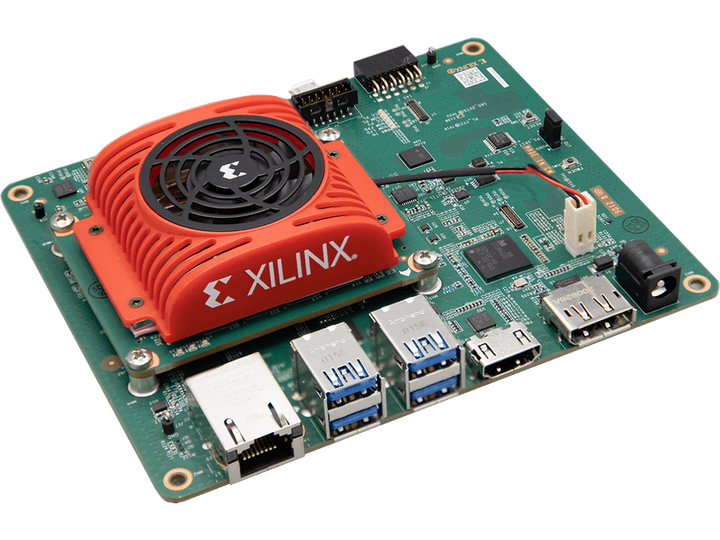
\includegraphics[width=0.8\textwidth]{./img/board}
\end{figure}

\pagebreak
\tableofcontents

\pagebreak
%-------------------------------------------------------------------------------
\section{Introduction and motivation}
\label{sec:intr-motiv}

\subsection{Documentation and guides}
\label{sec:documentation-guides}

\begin{itemize}
\item Board product information:\\ \url{https://www.xilinx.com/products/som/kria/kv260-vision-starter-kit.html}
\item SoC product information:\\ \url{https://www.xilinx.com/products/silicon-devices/soc/zynq-ultrascale-mpsoc.html}
\item Download page for the official Canonical Ubuntu releases for the board:\\ \url{https://ubuntu.com/download/amd-xilinx}
\item Xilinx official documentation:\\ \url{https://docs.xilinx.com/r/en-US/ug1089-kv260-starter-kit/Summary}
\item Atlassian documentation:\\ \url{https://xilinx-wiki.atlassian.net/wiki/spaces/A/pages/1641152513/Kria+K26+SOM}
\item Fixstar presentation (JP):\\  \url{https://speakerdeck.com/fixstars/fpga-seminar-12-fixstars-corporation-20220727}
\item Xilinx OpenAMP demo documentation:\\ \url{https://xilinx.github.io/kria-apps-docs/openamp/build/html/openamp\_landing.html}
\item Libmetal and OpenAMP official Xilinx documentation:\\ \url{https://docs.xilinx.com/r/en-US/ug1186-zynq-openamp-gsg/Introduction?tocId=GFruK4\_sY1eyu3jD9X1EuA}
\item Guide for KV260 board setup (JP):\\ \url{https://zenn.dev/ryuz88/articles/kv260\_setup\_memo\_ubuntu22}
\item Vitis IDE download page:\\ \url{https://www.xilinx.com/support/download/index.html/content/xilinx/en/downloadNav/vitis.html}
\end{itemize}

\pagebreak
% -------------------------------------------------------------------------------
\section{Boot Image Update}
\label{sec:boot-image-update}
In order to be able to boot a newer version of Linux, the
boot image of the board must be updated.

The procedure is available in \href{https://docs.xilinx.com/r/en-US/ug1089-kv260-starter-kit/Firmware-Update}{the official documentation},
but I will present it step by step here.

\subsection{Getting the new firmware}
\label{sec:getting-new-firmware}
A 2022 version of the board firmware is required in order to run the latest version of Ubuntu properly.

The image can be downloaded at \href{https://xilinx-wiki.atlassian.net/wiki/spaces/A/pages/1641152513/Kria+K26+SOM#Boot-FW-update-with-xmutil}{the atlassian page on the topic}.

\subsection{Reaching the board recovery tool}
\label{sec:reach-board-recov}
Now the firmware image is available, it is possible to update it using the boards recovery tool.
Here are the steps that must be taken in order to reach this tool and update the board:

\begin{itemize}
\item Connect the board to you machine via Ethernet.
\item Select the wired network as you connection (must be ``forced'', since it doesn't have internet access).
\item Set a fixed IP address for your machine, in the \verb|192.168.0.1/24| range, except the specific \verb|192.168.0.111|, which will be used by the board.
\item Using a web browser on your host machine, access \url{http://192.168.0.111}. You should now see the interface, as visible on the figure \ref{fig:recovery} below.
\item Now the downloaded file can be uploaded as a recovery image in the bottom-right section.
\end{itemize}

\begin{figure}[H]
  \centering
  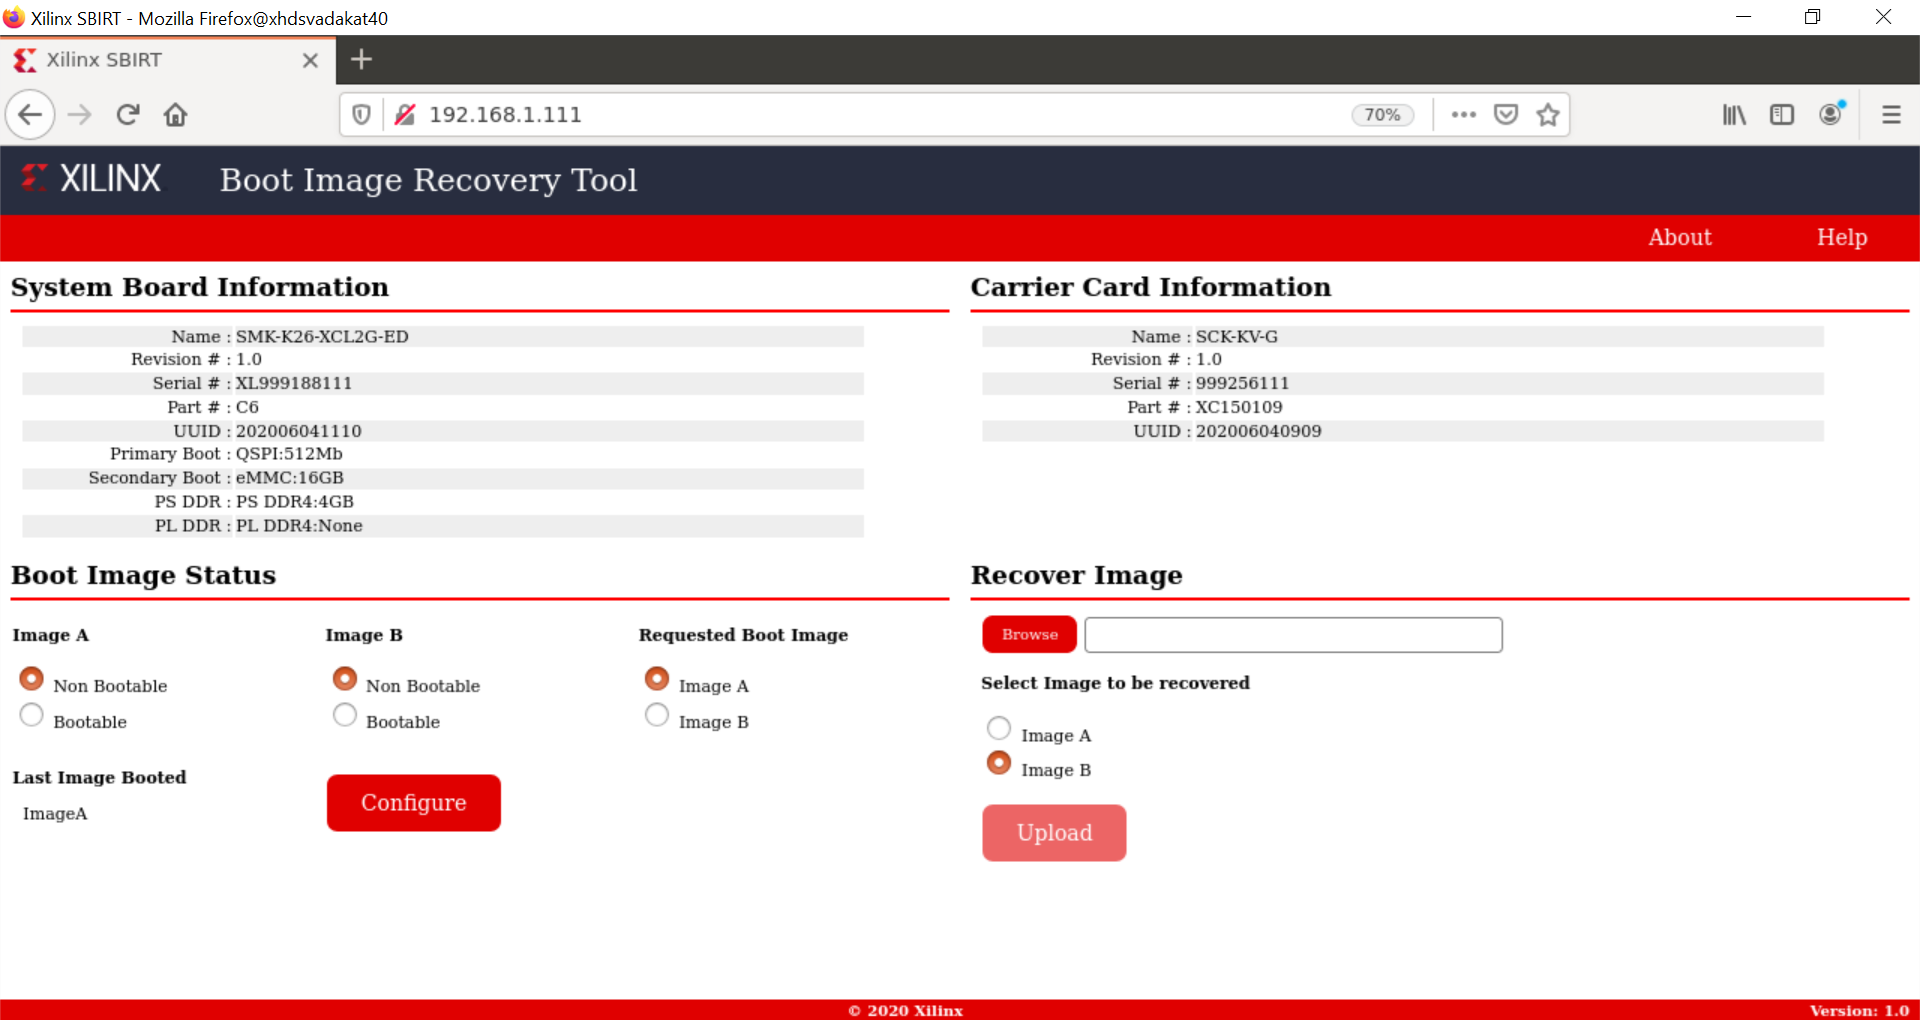
\includegraphics[width=0.7\textwidth]{./img/recovery.png}
  \caption{The recovery tool for the board, access from Firefox. We can see board information at the center, and the tools to upload the firmware at the bottom of the page.}
  \label{fig:recovery}
\end{figure}



%-------------------------------------------------------------------------------
\section{Ubuntu 22.04}
\label{sec:ubuntu-22.04}
\href{https://ubuntu.com/download/amd-xilinx}{An official Ubuntu image} is provided by Xilinx that allows the OS installation to be quick and
straightforward. Ubuntu is a common and easy to use distribution. Furthermore, it allows to install ROS2 as a package, which is most convenient
and will be done later in this guide.

One the image has been downloaded at Canonical's page (\url{https://ubuntu.com/download/amd-xilinx}), we can flash it onto the SD card.

\begin{tcolorbox}[colback=red!5!white,colframe=red!75!black]
  WARNING: The next part involve the \verb|dd| command writing on disks!!! \\
  As always with the dd command, you have to be VERY careful on what arguments you give. Selecting the wrong disk will result on the destruction of your data !! \\
  \underline{If you are unsure of what to do, seek assistance !}
\end{tcolorbox}


With the image available on you machine and a SD card visible as \verb|/dev/sda|\footnote{Again, it is critical to be 100\% certain that you are working with the correct device!}, one can simply run the \verb|dd| command as follow to write the image to a previously formatted drive (here \verb|/dev/sda|):
\begin{tcolorbox}
\begin{verbatim}
sudo dd if=iot-limerick-kria-classic-desktop-2204-x07-\
20230302-63.img of=/dev/sda status=progress bs=8M && sync
\end{verbatim}
\end{tcolorbox}

Once the SD card was flash, put back on the board and a micro-USB cable has been connected from the PC to the board, it is possible to
connect to the board in serial with an appropriate tool, for example picocom, as in the following example:
\begin{tcolorbox}
\begin{verbatim}
sudo picocom /dev/ttyUSB1 -b 115200
\end{verbatim}
\end{tcolorbox}

Once logged in, it is typically easier and more convenient to connect the board using SSH.
When the board is connected to the network, it is possible to know it's IP address with
the \verb|ip| command; then it is possible to connect to the board with ssh, as follow (example):
\begin{tcolorbox}
\begin{verbatim}
kria# ip addr

host# ssh ubuntu@192.168.4.11
\end{verbatim}
\end{tcolorbox}

\subsection{Proxy, DNS and root password}
\label{sec:proxy-dns}
An issue that can occur when connecting the board to the internet is the conflicting situation with
the school proxy.
Indeed, as the network at Nanzan University requires to go through a proxy, some DNS errors appeared.

Firstly, it is possible to set a DNS IP address in \verb|/etc/resolv.conf| by editing it and adding your favorite DNS, for example \verb|nameserver 1.1.1.1|
next to the other \verb|nameserver| entry.
\begin{tcolorbox}
\begin{verbatim}
sudo nano /etc/resolv.conf

sudo systemctl restart systemd-resolved
\end{verbatim}
\end{tcolorbox}

Secondly, it might become needed to setup the proxy for the school.

This can be done as follow, by exporting a https base proxy configuration containing you AXIA credentials, then
by consolidating the configuration for other types of connections in the \verb|bashrc|:
\begin{tcolorbox}
\begin{verbatim}
export https_proxy="http://<AXIA_username>:\
<AXIA_psw>@proxy.ic.nanzan-u.ac.jp:8080"

echo "export http_proxy=\""$https_proxy"\"" >> ~/.bashrc && \
echo "export https_proxy=\""$https_proxy"\"" >> ~/.bashrc && \
echo "export ftp_proxy=\""$https_proxy"\"" >> ~/.bashrc && \
echo "export no_proxy=\"localhost, 127.0.0.1,::1\"" \
>> ~/.bashrc
\end{verbatim}
\end{tcolorbox}

Finally, it might be convenient for the \verb|sudo| tool to not ask for the password all the time.
This change can be done by editing the sudoers file, and adding the parameter \verb|NOPASSWD|
at the ``sudo'' line:
\begin{tcolorbox}
\begin{verbatim}
sudo visudo

%sudo   ALL=(ALL:ALL) NOPASSWD: ALL
\end{verbatim}
\end{tcolorbox}

This is merely a convenience setup for devices staying at you desk. If
the board is meant to be used in any king of production setup, a password
should be set for making administration tasks.

With all of these settings, you should be able to update the software of your board
without any issues:
\begin{tcolorbox}
\begin{verbatim}
sudo apt-get update
sudo apt-get dist-upgrade
sudo reboot now
\end{verbatim}
\end{tcolorbox}


\subsection{Setting a static IP address}
\label{sec:setting-static-ip}
A static IP can be set by writing the following
configuration into your \verb|netplan| configuration file.

The name of the files might vary:
\begin{tcolorbox}
\begin{verbatim}
sudo nano /etc/netplan/50-cloud-init.yaml
\end{verbatim}
\end{tcolorbox}

You can then set the wanted IP as follow:
\begin{tcolorbox}
\begin{verbatim}
network:
  renderer: NetworkManager
  version: 2
  ethernets:
    eth0:
      addresses:
        - 192.168.11.103/24
      routes:
        - to: default
          via: 192.168.11.1
      nameservers:
        addresses:
          - 8.8.8.8
          - 1.1.1.1
\end{verbatim}
\end{tcolorbox}

Finally, the change in settings can be applied
as follow:
\begin{tcolorbox}
\begin{verbatim}
sudo netplan apply
\end{verbatim}
\end{tcolorbox}




\subsection{Extra: removing useless stuff}
\label{sec:extr-remov-usel}
As the desktop part is not used at all, there are some packages
that can be purges in order for the system to become more lightweight.

In particular, the main issue with Ubuntu systems is the forced integration of Snap.
Here are some step to try and remove all of that. These steps
take a lot of time though, but the system fan runs sensibly slower
without all of this stuff:
\begin{tcolorbox}
\begin{verbatim}
sudo systemctl disable snapd.service
sudo systemctl disable snapd.socket
sudo systemctl disable snapd.seeded.service
sudo snap list #show the installed package, remove then all:
sudo snap remove --purge firefox
sudo snap remove --purge gnome-3-38-2004
sudo snap remove --purge gnome-42-2204
sudo snap remove --purge gtk-common-themes
sudo snap remove --purge snapd-desktop-integration
sudo snap remove --purge snap-store
sudo snap remove --purge bare
sudo snap remove --purge core20
sudo snap remove --purge core22
sudo snap remove --purge snapd
sudo snap list # check that everything is uninstalled

sudo rm -rf /var/cache/snapd/
sudo rm -rf ~/snap
sudo apt autoremove --purge snapd

systemctl list-units | grep snapd
\end{verbatim}
\end{tcolorbox}

And here are some other stuff that can safely be removed too is the desktop is not to be used:
\begin{tcolorbox}
\begin{verbatim}
sudo apt-get autoremove --purge yaru-theme-icon \
fonts-noto-cjk yaru-theme-gtk vim-runtime \
ubuntu-wallpapers-jammy humanity-icon-theme

sudo apt-get autoclean
sudo reboot now
\end{verbatim}
\end{tcolorbox}

% -------------------------------------------------------------------------------
\section{Starting remoteproc}
\label{sec:starting-remoteproc}
One of the advantage of this board, as cited previously, is the presence of
multiple types of core (APU, MCU, FPGA) on the same chip.

The part we are focusing in this guide is the usage of both the APU, running
a Linux distribution and ROS2; and the MCU, running FreeRTOS and micro-ROS.

The communication between both side is meant to be done using shared memory, but
some extra setup is required.
This section will present how to setup and use as an example the \verb|remoteproc|
and RPMsg system.

\subsection{References}
\label{sec:referances}
This exact use-case is not exactly presented in the official documentation, but some
guides were found to eventually put together this procedure.

\begin{itemize}
\item \href{https://speakerdeck.com/fixstars/fpga-seminar-12-fixstars-corporation-20220727}{A slideshow (JP) from Fixstar employees} presents how
  to use the device tree to enable the communication between the cores.
\item \href{https://zenn.dev/ryuz88/articles/kv260_setup_memo_ubuntu22}{This blog article (JP)} shows all the major steps on how to enable the \verb|remoteproc|.
\end{itemize}


\subsection{DTO patching}
\label{sec:dto-patching}
The communication system and interaction from the Linux side towards the real-time capable core
is not enabled by default within the Ubuntu image provided by Xilinx.

Because of that, some modification of the device tree is required in order to have
the \verb|remoteproc| system to start.

Firstly, we need to get the original firmware device tree, converted
into a readable format (DTS):
\begin{tcolorbox}
\begin{verbatim}
sudo dtc /sys/firmware/fdt 2> /dev/null > system.dts
\end{verbatim}
\end{tcolorbox}

Then we can download and apply the patch that will allow us to use the \verb|remoteproc|:
\begin{tcolorbox}
\begin{verbatim}
wget https://gitlab.com/sunoc/xilinx-kria-kv260-\
documentation/-/raw/main/src/system.patch
patch system.dts < system.patch
\end{verbatim}
\end{tcolorbox}

As for the board to be able to reserve the correct amount of memory with the new settings, some
\verb|cma| kernel configuration is needed\footnote{The overlapping memory will not prevent the board to boot,
  but it disables the PWM for the CPU fan, which will then run at full speed, making noise.}:
\begin{tcolorbox}
\begin{verbatim}
sudo nano /etc/default/flash-kernel
LINUX_KERNEL_CMDLINE="quiet splash cma=512M cpuidle.off=1"
LINUX_KERNEL_CMDLINE_DEFAULTS=""
sudo flash-kernel
\end{verbatim}
\end{tcolorbox}

Now the DTS file has been modified, one can regenerate the binary and place it on the \verb|/boot| partition
and reboot the board:
\begin{tcolorbox}
\begin{verbatim}
dtc -I dts -O dtb system.dts -o user-override.dtb
sudo mv user-override.dtb /boot/firmware/
sudo reboot now
\end{verbatim}
\end{tcolorbox}

After rebooting, you can check the content of the \verb|remoteproc| system directory,
and a \verb|remoteproc0| device should be visible, as follow:
\begin{tcolorbox}
\begin{verbatim}
ls /sys/class/remoteproc/
#  remoteproc0
\end{verbatim}
\end{tcolorbox}

If it is the case, it means that the patch was successful and RPMsg is
ready to test with some example; however, in order for these examples
to be built, we need to setup Xilinx preferred IDE: Vitis.



% -------------------------------------------------------------------------------
\section{Vitis IDE}
\label{sec:vitis-ide}
This is the recommended IDE used to build software for the Xilinx boards.
It also include the tools to interact with the FPGA part, making the whole
software very large (around 200GB of disk usage).

The installer can be found on \href{https://www.xilinx.com/support/download/index.html/content/xilinx/en/downloadNav/vitis.html}{Xilinx download page}. You will need to get
a file named something like ``Xilinx\_Unified\_2022.2\_1014\_8888\_Lin64.bin''.

Vitis IDE installer is compatible with versions of Ubuntu, among other distributions,
but not officially yet for the 22.04 version.
Furthermore, the current install was tested on Pop OS, a distribution derived from Ubuntu.

This guide will present a guide that supposedly works for all distributions based on the newest
LTS from Ubuntu. For other Linux distributions or operating system, please refer to the official documentation.


\subsection{Install dependencies}
\label{sec:install-dependencies}
Some packages are required to be installed in order for the installation process to happen successfully:
\begin{tcolorbox}
\begin{verbatim}
sudo apt-get update
sudo apt-get install libncurses-dev \
ncurses-term \
ncurses-base \
ncurses-bin \
libncurses5 \
libtinfo5 \
libncurses5-dev \
libncursesw5-dev
\end{verbatim}
\end{tcolorbox}

Once this is done, the downloaded binary installer can be executed:
\begin{tcolorbox}
\begin{verbatim}
./Xilinx_Unified_2022.2_1014_8888_Lin64.bin
\end{verbatim}
\end{tcolorbox}

If it is not possible to execute it, make it executable with the \verb|chmod| command:
\begin{tcolorbox}
\begin{verbatim}
sudo chmod +x ./Xilinx_Unified_2022.2_1014_8888_Lin64.bin
\end{verbatim}
\end{tcolorbox}

From there you can follow the step-by-step graphical installer.
The directory chosen for the rest of this guide for the \verb|Xilinx| directory
is directly the \verb|\$HOME|, but the installation can be set elsewhere is needed.


% -------------------------------------------------------------------------------
\section{Building an example firmware for the Cortex R5F}
\label{sec:bulding-an-example}
As visible on the official \href{https://xilinx-wiki.atlassian.net/wiki/spaces/A/pages/1837006921/OpenAMP+Base+Hardware+Configurations\#Build-RPU-firmware}{Xilinx documentation about building a demo firmware}, this section will present the required steps for building a new firmware for the R5F core of our Kria board. The goal
here is to have a demonstration firmware running, able to use the RPMsg system to communicate with the Linux APU.

\subsection{Generating the platform configuration file}
\label{sec:gener-platf-conf}
In order to have the libraries and configurations in the IDE ready to be used for our board, we need to obtain configuration files, as presented in the 
\href{https://xilinx.github.io/kria-apps-docs/kv260/2022.1/build/html/docs/build_vitis_platform.html?highlight=xsa}{Xilinx guide for Kria and Vitis}. At the \href{https://github.com/Xilinx/kria-vitis-platforms}{dedicated repository}, we can have such configurations, but they required to be built.

\verb|Cmake|, \verb|tcl| and \verb|idn| will become needed in order to build the firmware.
As discussed in a thread on \href{https://support.xilinx.com/s/question/0D52E00006jrzsYSAQ/platform-project-cannot-be-created-on-vitis?language=en\_US}{Xilinx community forum}, \verb|libidn11| is specifically required, but creating a symbolic link from the current, 12 version works.

Here are the steps for building this configuration file:
\begin{tcolorbox}
\begin{verbatim}
sudo apt-get update
sudo apt-get install cmake tcl libidn11-dev \
libidn-dev libidn12 idn
sudo ln -s /usr/lib/x86_64-linux-gnu/libidn.so.12 \
/usr/lib/x86_64-linux-gnu/libidn.so.11

cd ~/Xilinx
git clone --recursive \
https://github.com/Xilinx/kria-vitis-platforms.git
cd kria-vitis-platforms/k26/platforms
export XILINX_VIVADO=/home/$USER/Xilinx/Vivado/2022.2/
export XILINX_VITIS=/home/$USER/Xilinx/Vitis/2022.2/
make platform PLATFORM=k26_base_starter_kit
\end{verbatim}
\end{tcolorbox}


%\pagebreak
\subsection{Setting up a new IDE project for the Kria board}
\label{sec:setting-up-new}
With the platform configuration files available, we can now use the IDE to generate a
new project for our board. The whole process will be described with screen captures and
captions.

\begin{figure}[H]
  \centering
  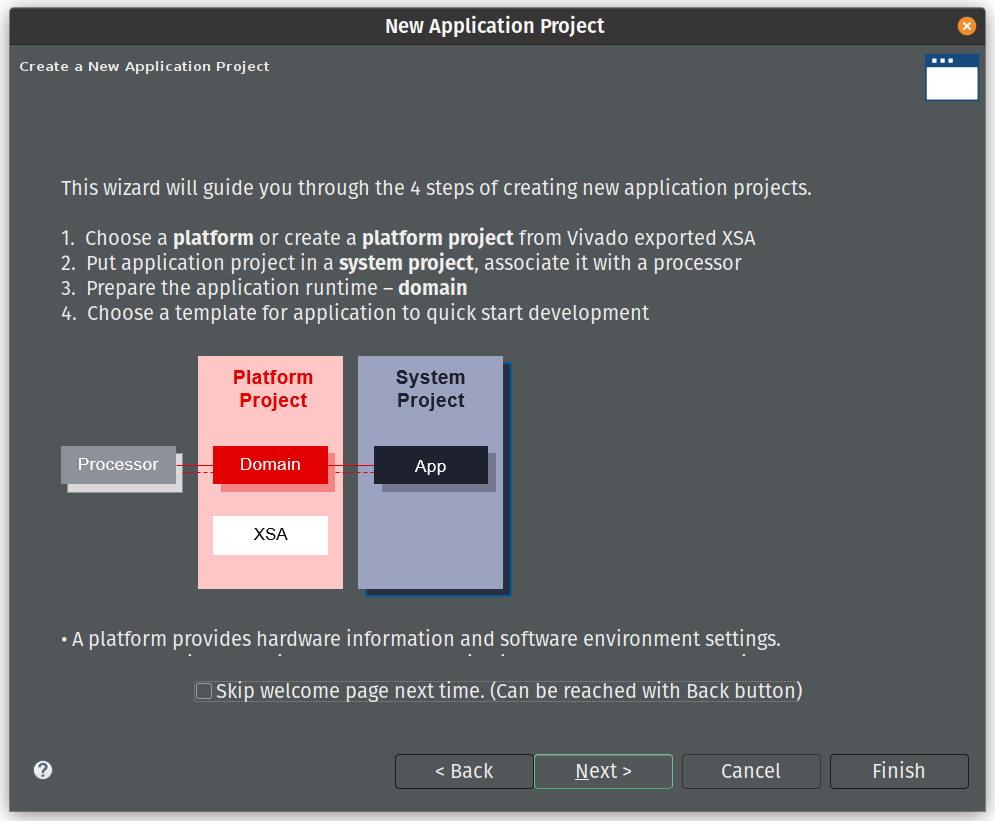
\includegraphics[width=0.6\textwidth]{./img/vitis_new/project1}
  \caption{We are starting with creating a ``New Application Project''. You should be greeted with this wizard window. Next.}
  \label{fig:project1}
\end{figure}

\begin{figure}[H]
  \centering
  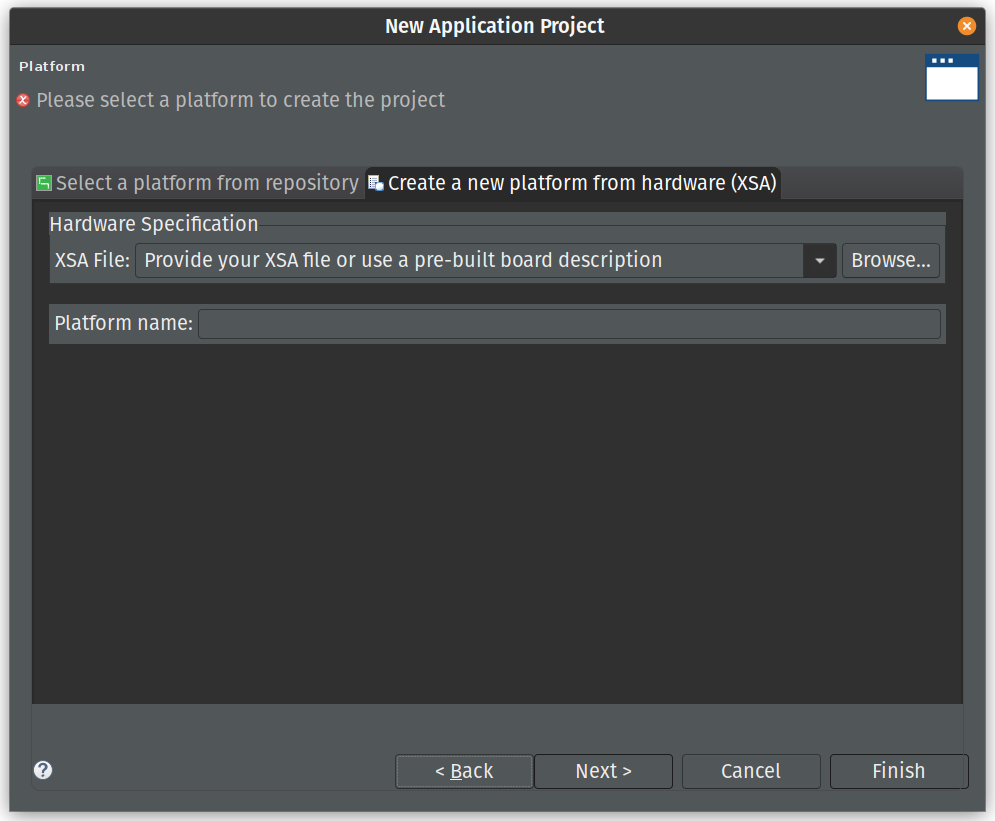
\includegraphics[width=0.7\textwidth]{./img/vitis_new/project2}
  \caption{For the platform, we need to get our build Kria configuration. In the ``Create a new platform...'' tab, click the ``Browse...'' button.}
  \label{fig:project2}
\end{figure}

\begin{figure}[H]
  \centering
  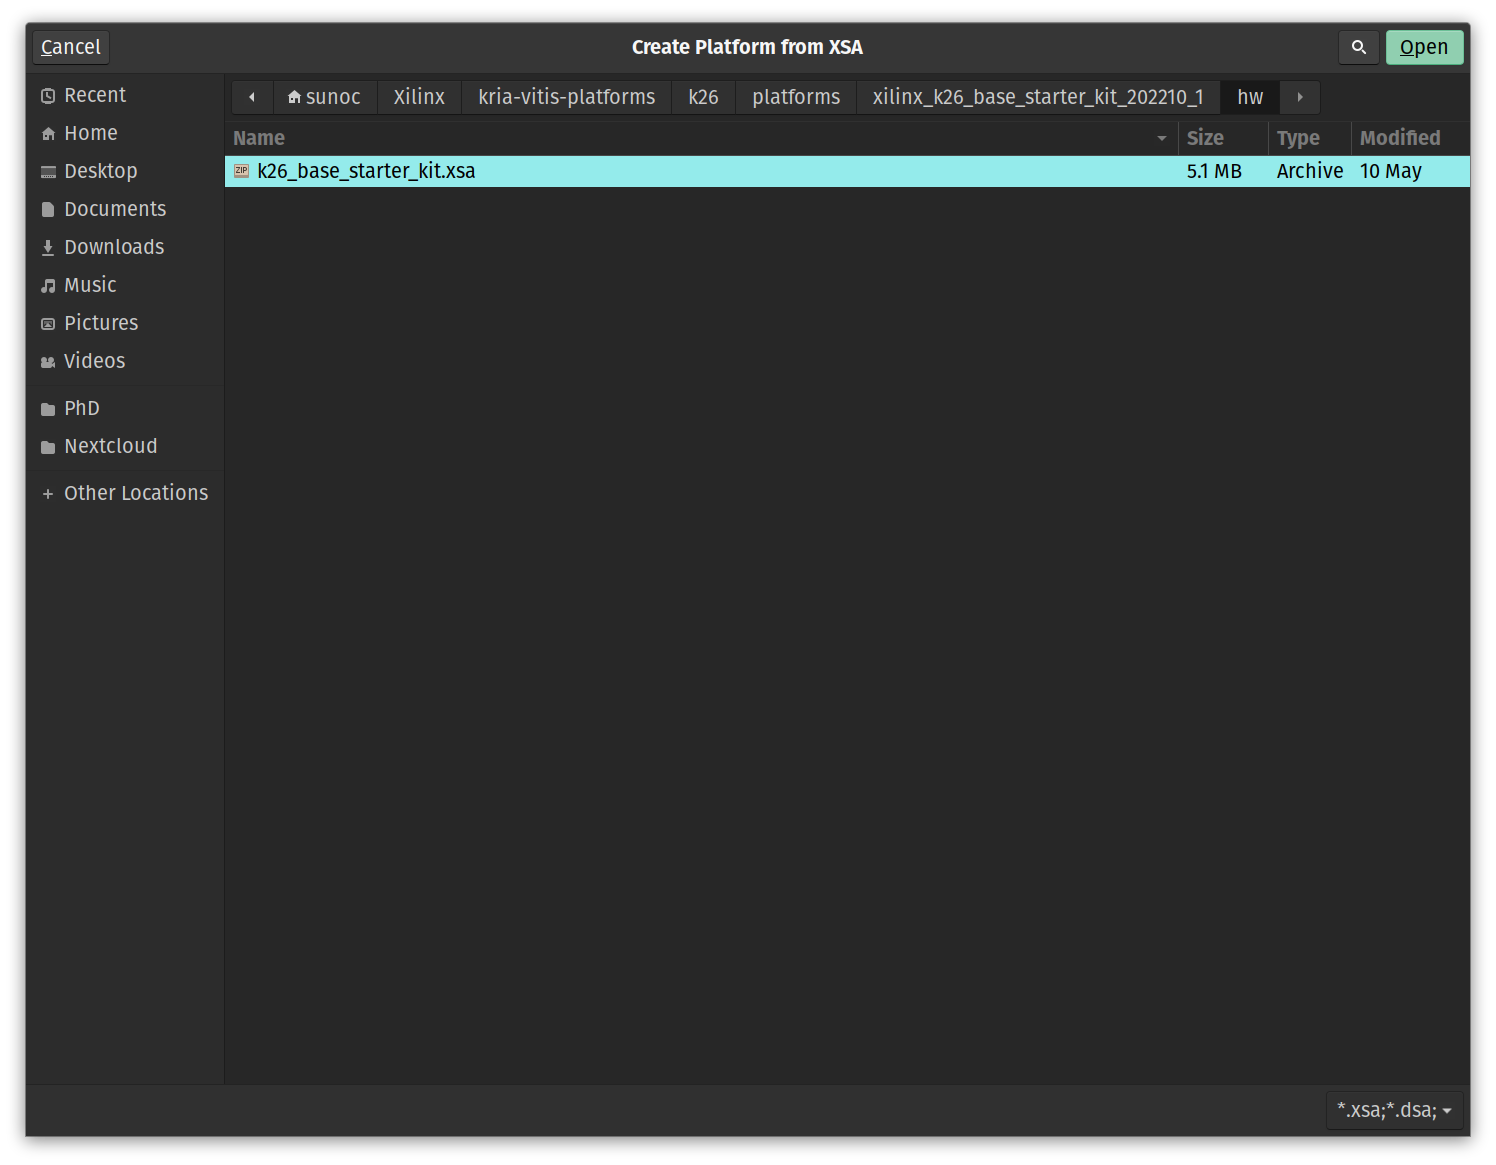
\includegraphics[width=0.7\textwidth]{./img/vitis_new/project3}
  \caption{In the file explorer, we should navigate in the ``k26'' directory, where the configuration file was build.
    From here we are looking for a ``.xsa'' file, located in a ``hw'' directory, as visible.}
  \label{fig:project3}
\end{figure}

\begin{figure}[H]
  \centering
  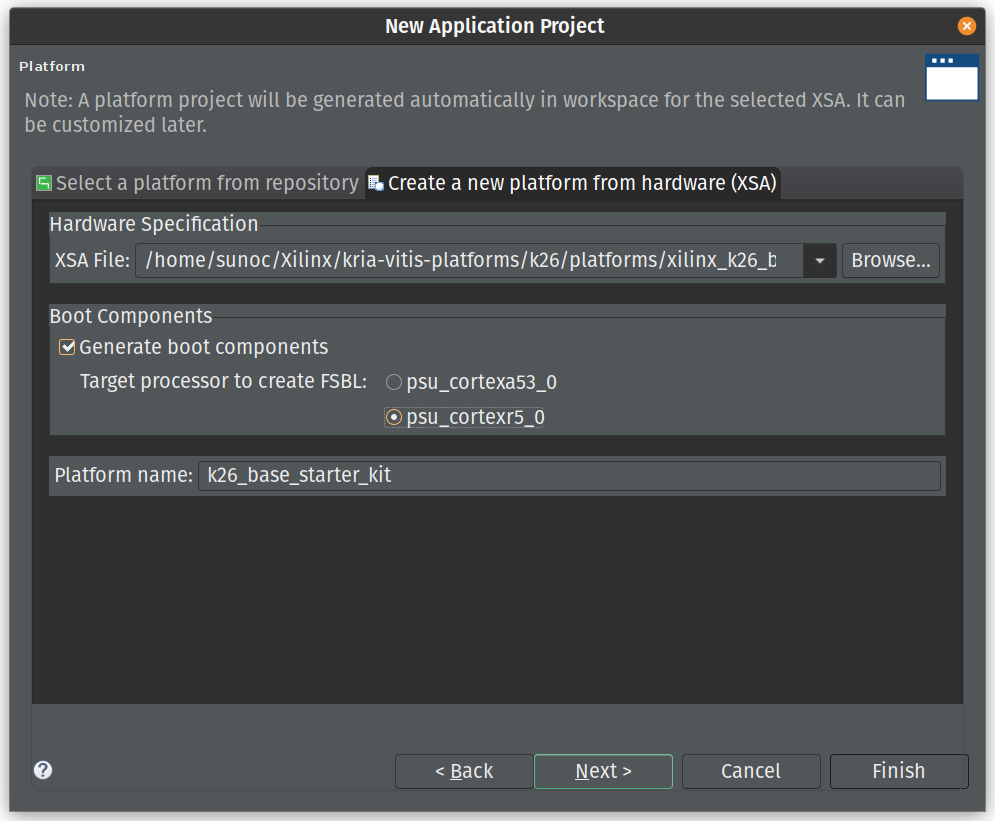
\includegraphics[width=0.7\textwidth]{./img/vitis_new/project4}
  \caption{With the configuration file loaded, we can now select a name for our platform, but most importantly, we have to select the ``psu\_cortex5\_0'' core
    as a target. The other, Cortex 53 is the APU running Linux.}
  \label{fig:project4}
\end{figure}

\begin{figure}[H]
  \centering
  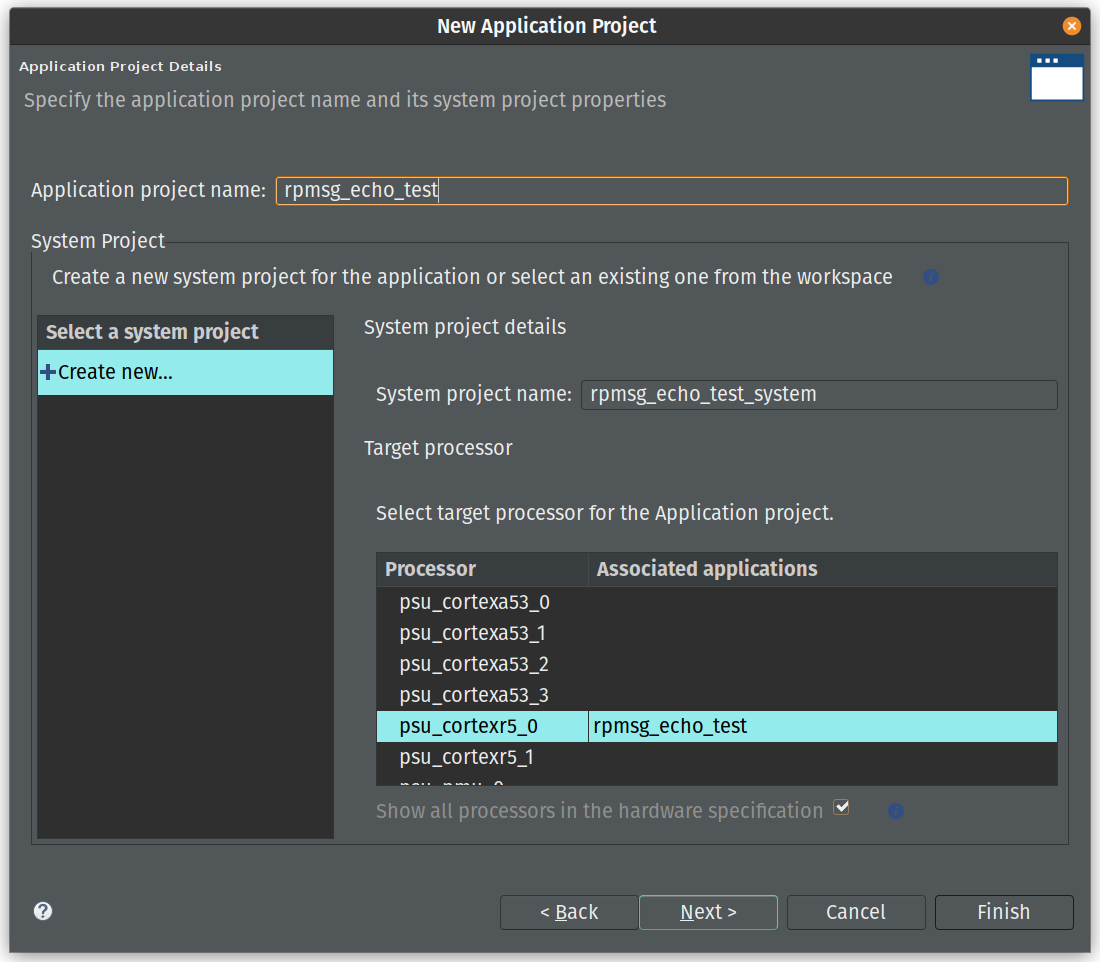
\includegraphics[width=0.7\textwidth]{./img/vitis_new/project5}
  \caption{In this next window, we can give a name to our firmware project. It is also critical here to select the core we want to build for.
    Once again, we want to use the ``psu\_cortex5\_0''.}
  \label{fig:project5}
\end{figure}

\begin{figure}[H]
  \centering
  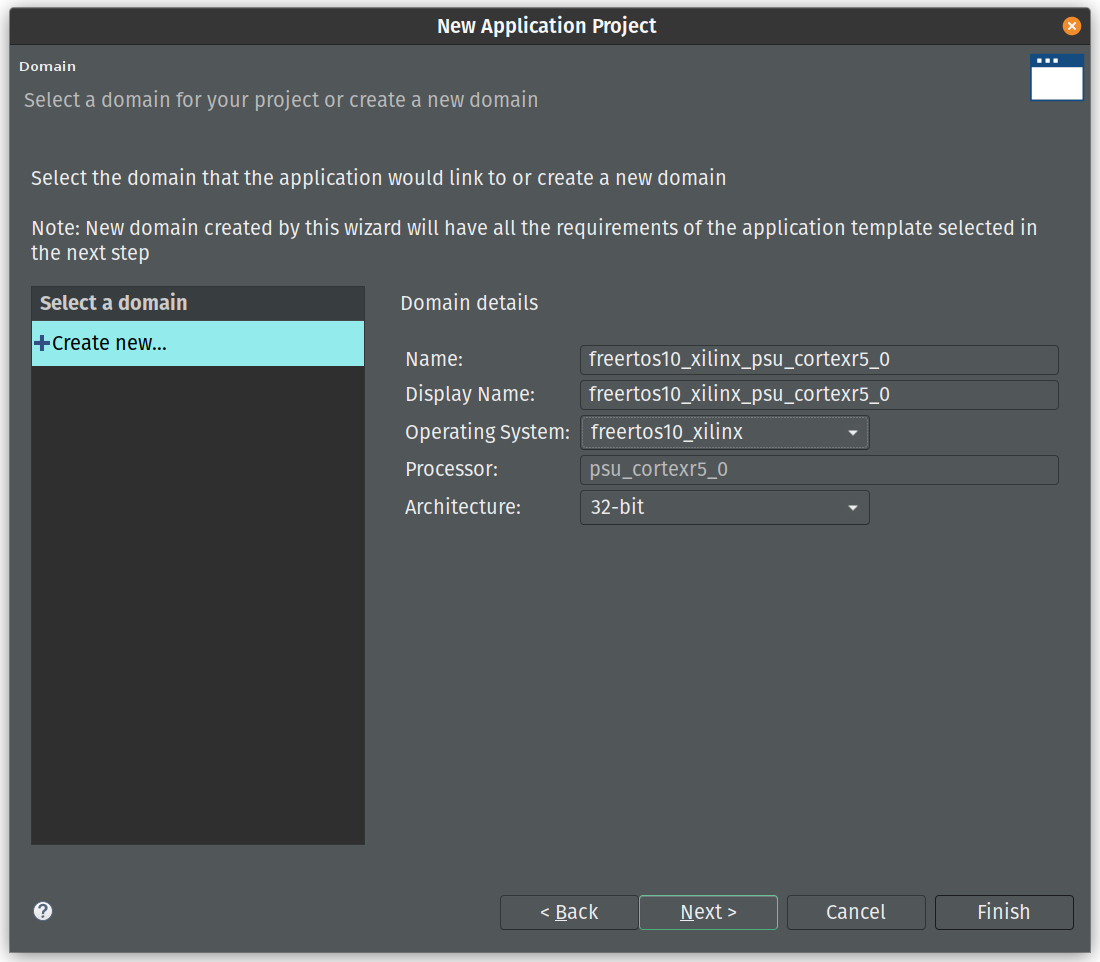
\includegraphics[width=0.7\textwidth]{./img/vitis_new/project6}
  \caption{Here, we want to select ``freertos10\_xilinx'' as our Operating System. The rest can remain unchanged.}
  \label{fig:project6}
\end{figure}

\begin{figure}[H]
  \centering
  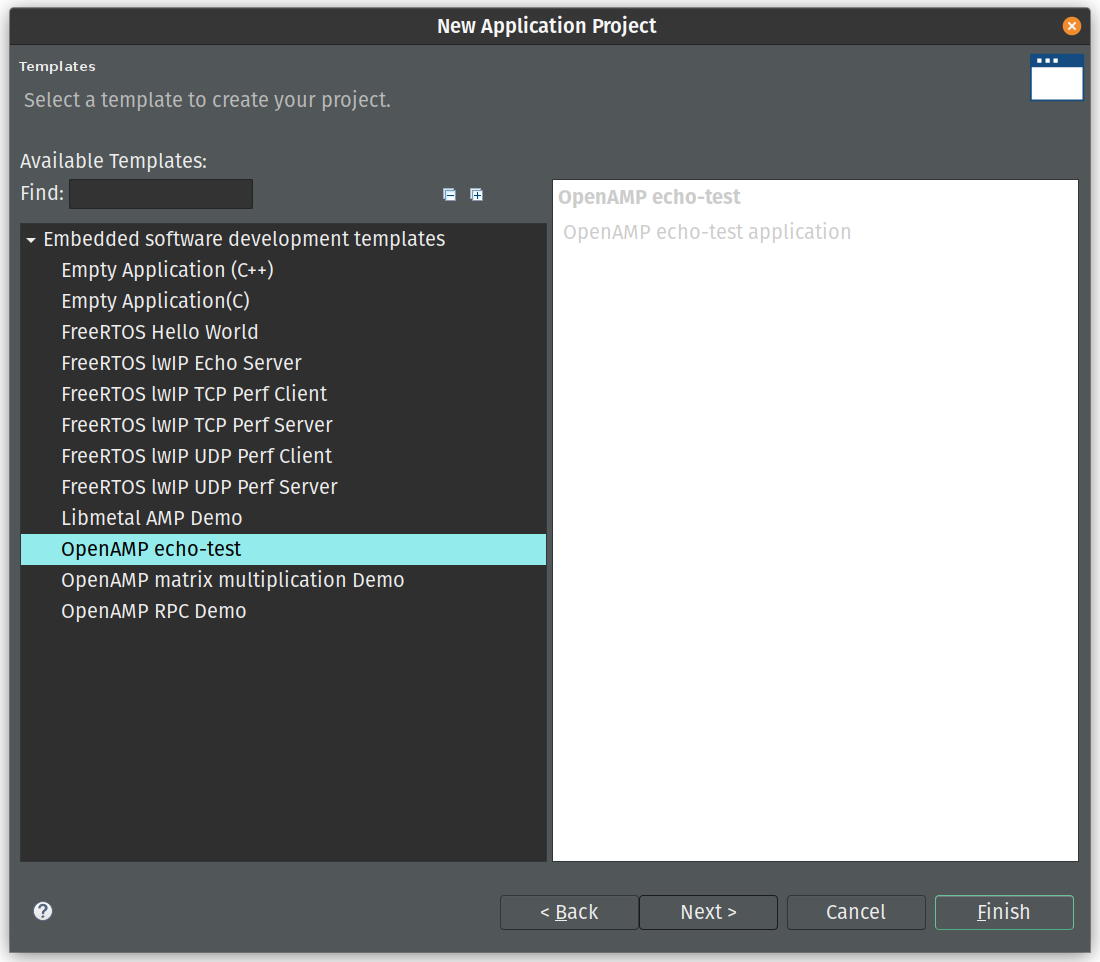
\includegraphics[width=0.7\textwidth]{./img/vitis_new/project7}
  \caption{Finally, we can select the demonstration template we are going to use; here we go with ``OpenAMP echo-test'' since we want to
    have some simple try of the RPMsg system. Finish.}
  \label{fig:project7}
\end{figure}


In the Xilinx documentation, it is made mention of the addresses setting that should be checked in the \verb|lscript.ld| file.
These valued look different from what could be set in the DTO for the Linux side, but they appear to
work for the example we are running:
\begin{tcolorbox}
\begin{verbatim}
psu_ddr_S_AXI_BASEADDR             0x3ed00000
psu_ocm_ram_1_S_AXI_BASEADDR       0xfffc0000
psu_r5_tcm_ram_0_S_AXI_BASEADDR    0x00000000
psu_r5_tcm_ram_1_S_AXI_BASEADDR    0x00020000
\end{verbatim}
\end{tcolorbox}



% -------------------------------------------------------------------------------
\section{Building and running an example program on the Linux side}
\label{sec:building-running-an}
In order to test the deployment of the firmware on the R5F side, and in particular
to test the RPMsg function, we need some program on the Linux side of the Kria
board to ``talk'' with the real-time side.

Some source is provided by Xilinx to build a demonstration software that does
this purpose: specifically interact with the demonstration firmware.

Here are the steps required to obtain the sources, and build the program.
As a reminder, this is meant to be done on the Linux running on the
Kria board, NOT on your host machine !
\begin{tcolorbox}
\begin{verbatim}
git clone https://github.com/Xilinx/meta-openamp.git
cd  meta-openamp
git checkout xlnx-rel-v2022.2
cd  .//recipes-openamp/rpmsg-examples/rpmsg-echo-test
make
sudo ln -s $(pwd)/echo_test /usr/bin/
\end{verbatim}
\end{tcolorbox}



% -------------------------------------------------------------------------------
\section{WIP::: Loading a new firmware from Linux}
\label{sec:loading-new-firmware}
This is a work in progress.

These instructions are useful to upload and start the firmware
on the R5F from the Linux, but there are some issues.
This will be fixed eventually.
\begin{tcolorbox}
\begin{verbatim}
sudo -s
cp image_echo_test /lib/firmware
echo image_echo_test  > /sys/class/remoteproc/\
remoteproc0/firmware
echo start > /sys/class/remoteproc/remoteproc0/state
echo_test
echo stop > /sys/class/remoteproc/remoteproc0/state
\end{verbatim}
\end{tcolorbox}



% -------------------------------------------------------------------------------
\section{Building the micro-ROS static library}
\label{sec:building-micro-ros}
In this section, the goal is to build the micro-ROS library in order to be
able to integrate the micro-ROS function into our Cortex R5F firmware.
All of this should be done via cross-compiling on a host machine, however
it is most common in the guides about micro-ROS to build the firmwares and libraries within a Docker,
so we can have access of the ROS environment without installing it on my machine.
One can simply run this command to summon a ROS2 Docker\footnote{If Docker is not set up on your machine, you can follow the guide on \href{https://docs.docker.com/engine/install/ubuntu/}{the official website}. When you can successfully run the ``hello-world'' container, you are good to go.} with the wanted version, but first we also need to check the cross-compilation tools.

These are provided with the Vitis IDE, installed earlier in this guide, but
you should check if the path to the binaries are correct:

\begin{tcolorbox}
\begin{verbatim}
sudo find / -name 'armr5-none-eabi-gcc'
\end{verbatim}
\end{tcolorbox}

The return should look something like this:\\
\verb|/home/sunoc/Xilinx/Vitis/2022.2/gnu/armr5/lin/|\\
\verb|gcc-arm-none-eabi/bin/armr5-none-eabi-gcc|

You can then re-use some part of that path and run the following commands to start the
Docker container with access to the toolchain for ARM R5:
\begin{tcolorbox}
\begin{verbatim}
toolchain="/home/sunoc/Xilinx/Vitis/2022.2/gnu/\
armr5/lin/gcc-arm-none-eabi/"
docker run -d --name ros_build -it --net=host \
-v /dev:/dev \
-v $toolchain:/armr5-toolchain \
--privileged ros:humble
docker exec -it ros_build bash
\end{verbatim}
\end{tcolorbox}


Now we are in the ROS2 container, we can build the micro-ROS firmware as presented in the \href{https://micro.ros.org/docs/tutorials/advanced/create\_custom\_static\_library}{dedicated micro-ROS guide}:
\begin{tcolorbox}
\begin{verbatim}
ln -s /armr5-toolchain/armrm-xilinx-eabi/usr/include/c++/11.2.0/arm-xilinx-eabi/arm/ /usr/include/c++/11/
ln -s /armr5-toolchain/armrm-xilinx-eabi/usr/include/c++/11.2.0/arm-xilinx-eabi/bits/* /usr/include/c++/11/bits/
ln -s /armr5-toolchain/armrm-xilinx-eabi/usr/include/c++/11.2.0/arm-xilinx-eabi/ext/* /usr/include/c++/11/ext/
ln -s /armr5-toolchain/armrm-xilinx-eabi/usr/include/c++/11.2.0/arm-xilinx-eabi/thumb/ /usr/include/c++/11/

# link the libraries
ln -s /armr5-toolchain/x86_64-oesdk-linux/lib/* /lib

# ignore the warnings for the next command:
ln -s /armr5-toolchain/armrm-xilinx-eabi/usr/include/* /usr/include/

# overriding some of the headers
ln -fs /armr5-toolchain/armrm-xilinx-eabi/usr/include/ctype.h /usr/include/
ln -fs /armr5-toolchain/armrm-xilinx-eabi/usr/include/locale.h /usr/include/
ln -fs /armr5-toolchain/armrm-xilinx-eabi/usr/include/pthread.h /usr/include/
ln -fs /armr5-toolchain/armrm-xilinx-eabi/usr/include/threads.h /usr/include/

# don't wanna use the x86 __locale header
mv /usr/include/x86_64-linux-gnu/bits/types/__locale_t.h /usr/include/x86_64-linux-gnu/bits/types/BKP__locale_t.h
mv /usr/include/x86_64-linux-gnu/bits/types/locale_t.h /usr/include/x86_64-linux-gnu/bits/types/BKP_locale_t.h
ln -s /armr5-toolchain/armrm-xilinx-eabi/usr/include/sys/_locale.h /usr/include/c++/11/bits/
mkdir /usr/include/c++/11/bits/types/
ln -s /armr5-toolchain/armrm-xilinx-eabi/usr/include/sys/_locale.h /usr/include/c++/11/bits/types/locale_t.h


. /opt/ros/$ROS_DISTRO/setup.bash

mkdir microros_ws
cd microros_ws
git clone -b $ROS_DISTRO \
https://github.com/micro-ROS/micro_ros_setup.git \
src/micro_ros_setup

sudo apt update && \
sudo apt-get -y install python3-pip wget nano

sudo rosdep fix-permissions
rosdep update
rosdep install --from-paths src --ignore-src -y

colcon build
. ./install/local_setup.bash

# using my fork for the ament_cmake repository
sed -i 's/ament\/ament_cmake/sunoc\/ament_cmake/g' ./install/micro_ros_setup/config/generate_lib/dev_ros2_packages.txt
sed -i 's/ament\/ament_cmake/sunoc\/ament_cmake/g' ./src/micro_ros_setup/config/generate_lib/dev_ros2_packages.txt
sed -i 's/raw.githubusercontent.com\/ros2\/ros2\/humble\/ros2.repos/gitlab.com\/sunoc\/xilinx-kria-kv260-documentation\/-\/snippets\/2548852\/raw\/main\/ros2.repos/g' ./src/micro_ros_setup/scripts/create_ws.sh

# same for the ament_index repository
sed -i 's/ament\/ament_index/sunoc\/ament_index/g' ./install/micro_ros_setup/config/generate_lib/dev_ros2_packages.txt
sed -i 's/ament\/ament_index/sunoc\/ament_index/g' ./src/micro_ros_setup/config/generate_lib/dev_ros2_packages.txt


ros2 run micro_ros_setup create_firmware_ws.sh generate_lib

touch custom_r5f_toolchain.cmake
touch custom_r5f_colcon.meta
\end{verbatim}
\end{tcolorbox}

From there we will need some configuration files specifically for
our Cortex R5F. The two following settings are required in order to build our library.


Here is a configuration that should work for you \verb|my_custom_toolchain.cmake|

WIP: make this available as a downloadable file form my git repo.
\begin{tcolorbox}
\verbatiminput{src/my_custom_toolchain.cmake}
\end{tcolorbox}

And here is a configuration for the \verb|my_custom_colcon.meta|.

WIP: make this available as a downloadable file form my git repo.
\begin{tcolorbox}
\verbatiminput{src/my_custom_colcon.meta}
\end{tcolorbox}


Now we have both our configuration wiles, we can build the library with the following ros2 command:
\begin{tcolorbox}
\begin{verbatim}
ln -s /armr5-toolchain/armrm-xilinx-eabi/usr/include/c++/11.2.0/ /usr/include/c++/
ln -s /armr5-toolchain/armrm-xilinx-eabi/usr/include/c++/11.2.0/arm-xilinxmllibarmv5tehard-eabi/bits/c++config.h /armr5-toolchain/armrm-xilinx-eabi/usr/include/c++/11.2.0/bits/
ln -s /usr/include/dlfcn.h /armr5-toolchain/armrm-xilinx-eabi/usr/include/



ros2 run micro_ros_setup build_firmware.sh \
$(pwd)/custom_r5f_toolchain.cmake $(pwd)/custom_r5f_colcon.meta
\end{verbatim}
\end{tcolorbox}

Then, back on the host machine, we can download the static library and the include files:
\begin{tcolorbox}
\begin{verbatim}
mkdir /home/$USER/Xilinx/\
workspace/openamp_echo_demo/microros_lib

scp ubuntu@192.168.11.4:/microros_ws/firmware/build/* \
/home/$USER/Xilinx/workspace/openamp_echo_demo/microros_lib/
\end{verbatim}
\end{tcolorbox}



% -------------------------------------------------------------------------------
\section{Including the micro-ROS static library in a project}
Now we have a Vitis demonstration project available and the \verb|libmicroros| static library
available, we can combine both by including this library into our Kria project.

Many parameters are available to be set up in the IDE for the compilation toolchain, but here is
a setup that worked to have the IDE to recognize the include files and to be able to use them
for compiling the firmware.

\label{sec:including-micro-ros}
\begin{figure}[H]
  \centering
  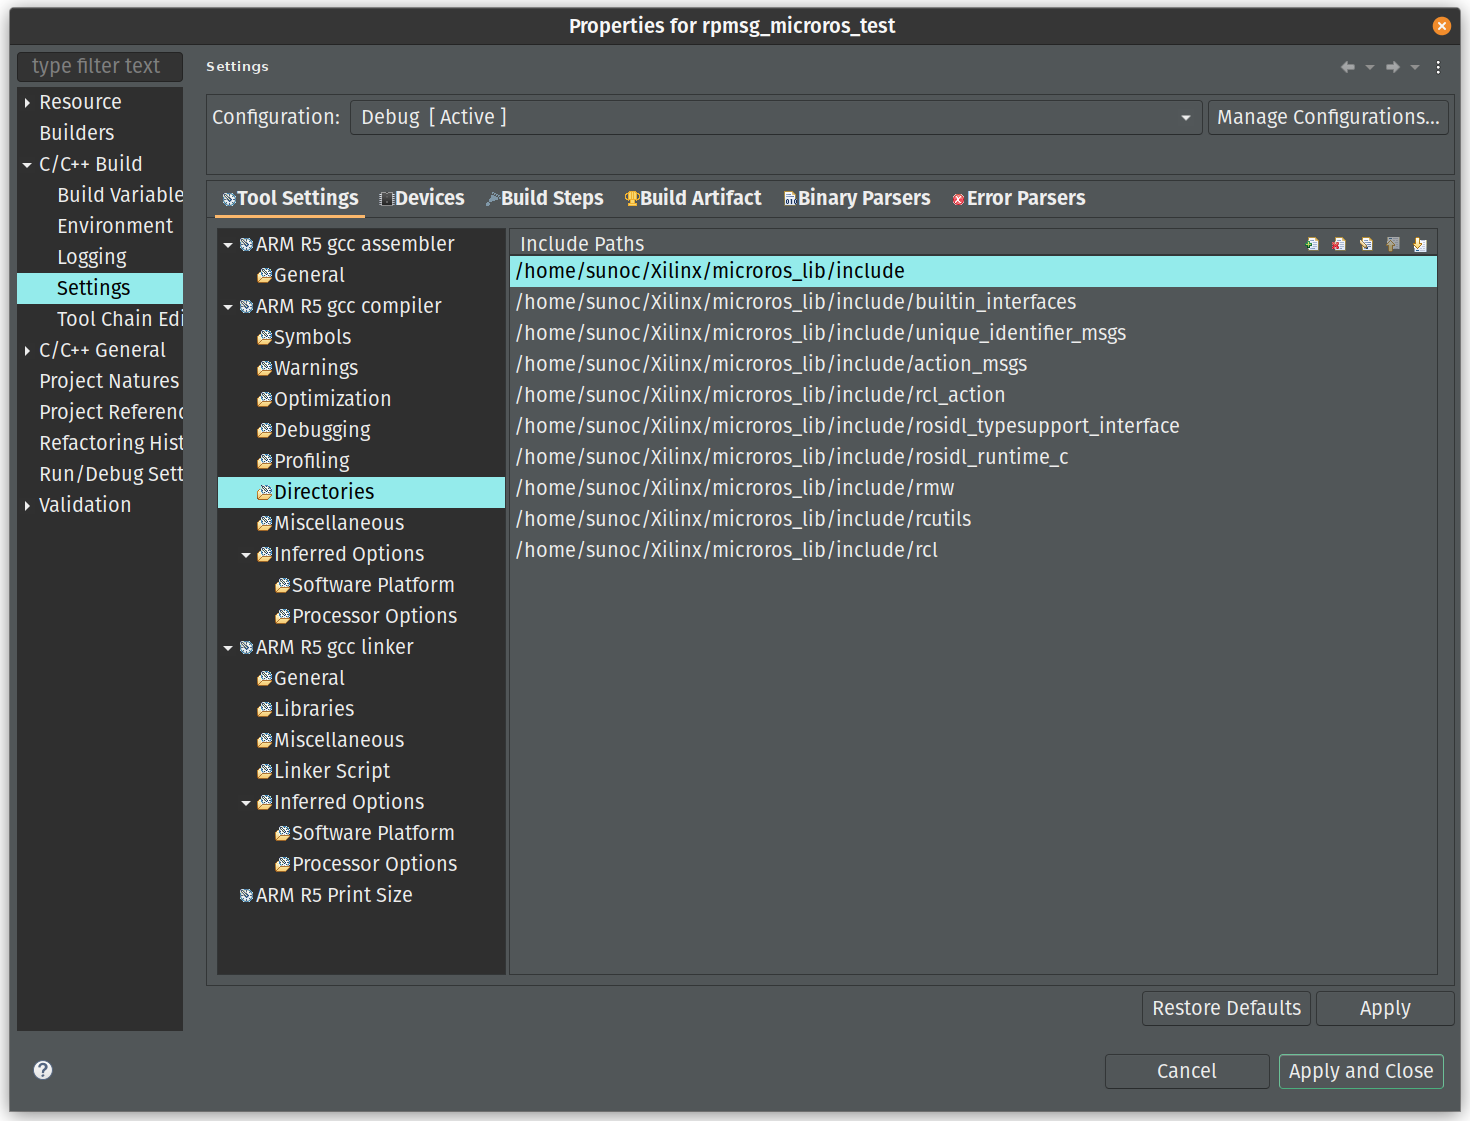
\includegraphics[width=0.7\textwidth]{./img/vitis_new/include}
  \caption{Firstly, in the ``C/C++ Build'' settings of your firmware project, under the ``Settings'' menu, you should find the gcc compiler
    ``Directories''. In here you should add the ``include'' directory of your library. Be careful however, if your include files are in
  a second layer of directory (as it is the case for libmicroros) you will need to include each sub-directory individually.}
  \label{fig:include1}
\end{figure}

\begin{figure}[H]
  \centering
  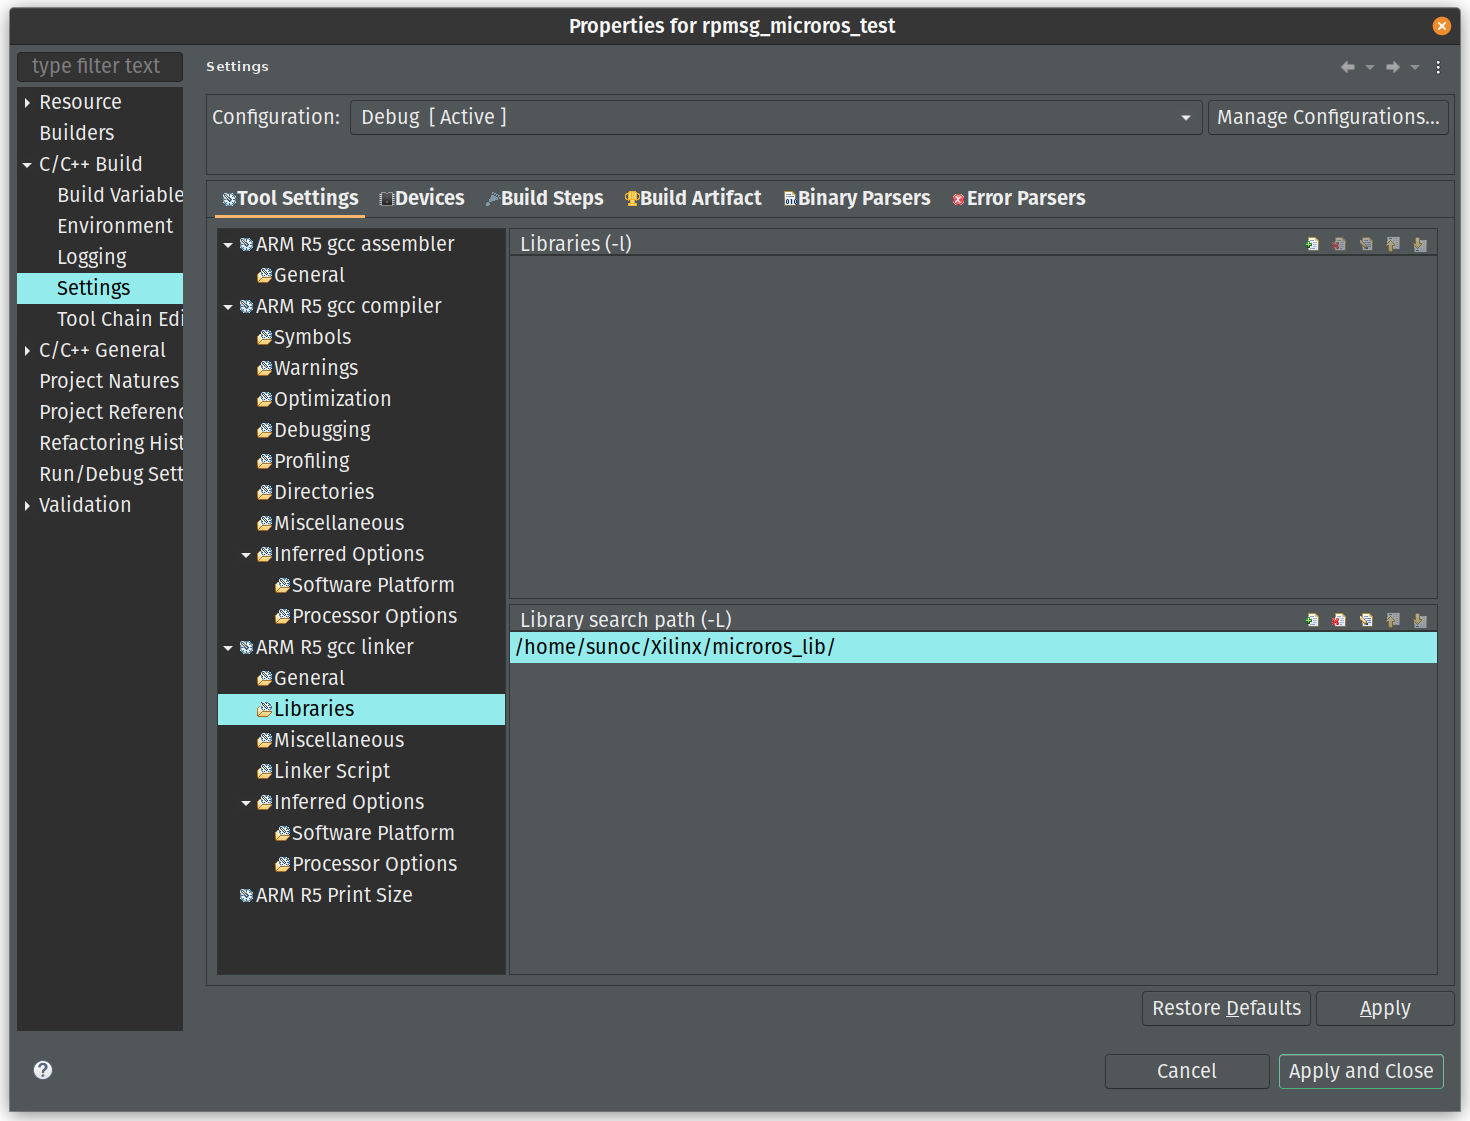
\includegraphics[width=0.7\textwidth]{./img/vitis_new/include2}
  \caption{Secondly, in the gcc linkers ``Libraries'', you can add the top level directory of your library. In our case, it is the
    directory that contains both the ``include'' directory added earlier, and also the ``libmicroros.a'' file.}
  \label{fig:include2}
\end{figure}

With both of these setup in your project, you should be able to include the following micro-ROS libraries into your project:
\begin{tcolorbox}
\begin{verbatim}
#include <rcl/rcl.h>
#include <rcl/error_handling.h>
#include <rclc/rclc.h>
#include <rclc/executor.h>
\end{verbatim}
\end{tcolorbox}


% -------------------------------------------------------------------------------
\pagebreak
\section{ROS2}
\label{sec:ros2}
As an Ubuntu distribution is installed on the board, the installation of ROS2 can be done
in a standard way, using the repository.

An \href{https://docs.ros.org/en/humble/Installation/Ubuntu-Install-Debians.html}{official documentation}
is provided with ROS2 themselves with a step-by-step guide on how to install
ROS2 on a Ubuntu system\footnote{The curl command from the guide does not work through the school proxy,
  but the command wget used instead does work. The key is then moved to the correct spot with mv}.
We will follow this guide here.

Firstly, we need to update the locals,  enable the universe Ubuntu repository, get the key and add the repository for ROS2. This can be done as follow:

\begin{tcolorbox}
\begin{verbatim}
locale  # check for UTF-8
sudo apt update && sudo apt install -y locales
sudo locale-gen en_US en_US.UTF-8
sudo update-locale LC_ALL=en_US.UTF-8 LANG=en_US.UTF-8
export LANG=en_US.UTF-8
locale  # verify settings
sudo apt install -y software-properties-common
sudo add-apt-repository universe
sudo apt update && sudo apt install -y curl wget
wget https://raw.githubusercontent.com/ros/rosdistro/\
master/ros.key
sudo mv ros.key /usr/share/keyrings/ros-archive-keyring.gpg
\end{verbatim}
\end{tcolorbox}


This is a one-liner to add the ROS2 repository:

\begin{tcolorbox}
\begin{verbatim}
echo "deb [arch=$(dpkg --print-architecture) \
signed-by=/usr/share/keyrings/ros-archive-keyring.gpg] \
http://packages.ros.org/ros2/ubuntu $(. \
/etc/os-release && echo $UBUNTU_CODENAME) main" | \
sudo tee /etc/apt/sources.list.d/ros2.list > /dev/null
\end{verbatim}
\end{tcolorbox}

It is then possible to install ROS2\footnote{This command installs a complete ``desktop'' version of ROS2. If space is a constraint, different, less complete packages can be install. Please refer to the official documentation about it.} as follow:

\begin{tcolorbox}
\begin{verbatim}
sudo apt update
sudo apt upgrade -y
sudo apt install -y ros-humble-desktop \
ros-humble-ros-base \
python3-argcomplete \
ros-dev-tools
\end{verbatim}
\end{tcolorbox}

Once installed, it is possible to test the system with a provided example. You need to open two terminals and log wish SSH onto the board, then running respectively:

\begin{tcolorbox}
\begin{verbatim}
source /opt/ros/humble/setup.bash
ros2 run demo_nodes_cpp talker
\end{verbatim}
\end{tcolorbox}



\begin{tcolorbox}
\begin{verbatim}
source /opt/ros/humble/setup.bash
ros2 run demo_nodes_py listener
\end{verbatim}
\end{tcolorbox}


You should be able to see the first terminal sending "Hello world" messages, and the second one receiving then.


% -------------------------------------------------------------------------------
\section{ROS2 in a container}
\label{sec:ros2-container}
As it is used to test and build micro-ROS configurations, running ROS2 in a Docker container is a great way to have a reproducible configuration
of you system. This part of the guide will present how to install Docker on the Kria board and then how to use it to deploy the latest
version of ROS2.

\subsection{Installing docker}
\label{sec:installing-docker}
It is possible to have a version of Docker installed simply by using the available repository, but since we are on Ubuntu, a PPA is available
from Docker in order to have the most up-to-date version.
Following \href{https://docs.docker.com/engine/install/ubuntu/#install-using-the-repository}{the official documentation}, the following steps can be taken to
install the latest version of Docker on a Ubuntu system.
The last command is meant to test the install. If everything went smoothly, you should see something similar to what is presented on the figure \ref{fig:hello-docker} below:
\begin{tcolorbox}
\begin{verbatim}
sudo apt-get update
sudo apt-get install ca-certificates curl gnupg
sudo install -m 0755 -d /etc/apt/keyrings
curl -fsSL https://download.docker.com/linux/ubuntu/gpg | \
sudo gpg --dearmor -o /etc/apt/keyrings/docker.gpg

sudo chmod a+r /etc/apt/keyrings/docker.gpg

echo \
  "deb [arch="$(dpkg --print-architecture)" \
  signed-by=/etc/apt/keyrings/docker.gpg] \
  https://download.docker.com/linux/ubuntu \
  "$(. /etc/os-release && \
  echo "$VERSION_CODENAME")" stable" | \
  sudo tee /etc/apt/sources.list.d/docker.list > /dev/null

sudo apt-get update
sudo apt-get install docker-ce docker-ce-cli \
  containerd.io docker-buildx-plugin docker-compose-plugin
sudo usermod -aG docker $USER
newgrp docker

docker run hello-world
\end{verbatim}
\end{tcolorbox}

\begin{figure}[H]
  \centering
  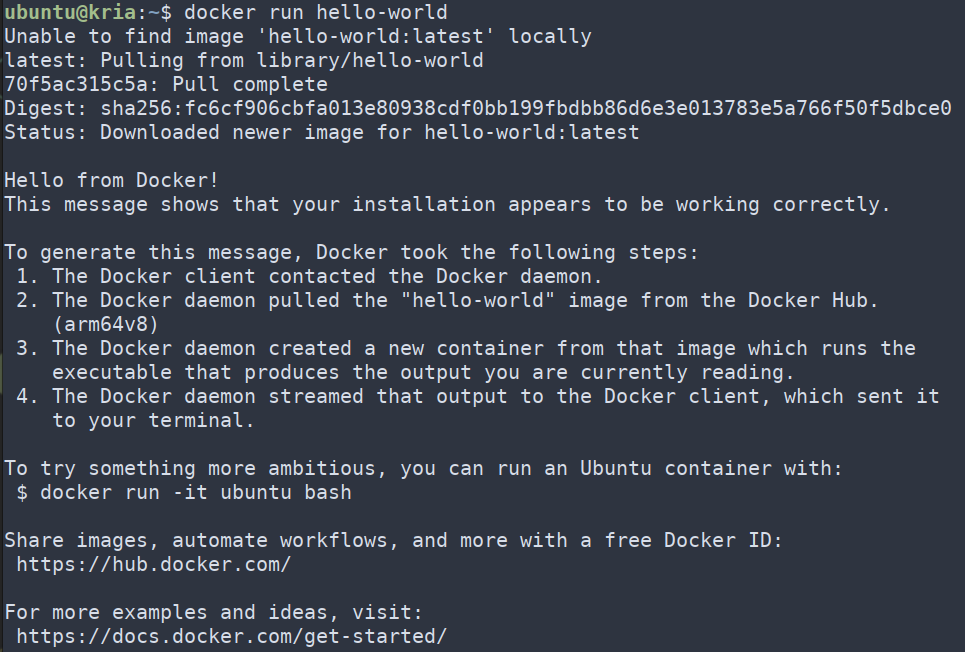
\includegraphics[width=0.9\textwidth]{./img/hello-docker.png}
  \caption{The return of a successful run of the ``hello world'' test Docker container}
  \label{fig:hello-docker}
\end{figure}

\subsection{Calling a ROS2 container}
\label{sec:call-ros2-cont}
The following commands will pull a ROS container, version \verb|humble|, and name it \verb|ros_build|.
A key part for having access to the interfaces (serial) is the mapping of whole the \verb|/dev| of  the host machine to the
internal \verb|/dev|. \footnote{Note that this is an example and this situation can become a security issue. It would be a better practice
in a production environment to map only the devices that are actually in use.}
With the second command, we can execute \verb|bash|, as a way to open a terminal to the ``inside'' of the container.
\begin{tcolorbox}
\begin{verbatim}
sudo docker run -d --name ros_build -it --net=host -v \
     /dev:/dev --privileged ros:humble
sudo docker exec -it ros_build bash
\end{verbatim}
\end{tcolorbox}

From there, it becomes possible to simply use ROS2 as you would for a bare-metal install, and as presented in the section \ref{sec:ros2}.

\end{document}